\chapter{Konzepte}
\label{ch:chapter04}
In diesem Kapitel wird darauf eingegangen, wie vorgegangen wurde, um verschiedene Konzepte zu entwickeln.
Dabei werden die vorher erwähnten Befragungen (\ref{ch:Recherche}) verwendet, um eine Lösung für die individuellen Probleme zu entwickeln.
Zudem wird der Stand der Technik betrachtet und ein Vergleich mit den Datenbankstrukturen gezogen.
Dies wird getan, da diese eine ähnliche Struktur wie die Berechtigungsstruktur der Helvetia haben. 
Anschließend werden die Probleme aus den Befragungen quantifiziert, um daraus die verschiedenen Konzepte zu entwickeln.

\section{Konzeptentwicklung}
\label{sec:chapter04:Konzeptentwicklung}
In diesen Unterkapiteln wird betrachtet, was der Stand der Technik ist.
Dabei werden die Sicherheitsmaßnahmen von \ac{IAM} erläutert sowie berücksichtigt, dass es nicht die eine Lösung für das Problem gibt.
Zudem wird auch erläutert wie die Berechtigungsstruktur innerhalb von Datenbanken funktioniert, um diese als einen Vergleich zu nutzen.  

\subsection{Stand der Technik}
\label{sec:chapter04:Stand}
In der Welt von Cloud Computing wird \ac{IAM} als Sicherheitsmaßnahme verwendet.
Dabei wird mittels \ac{IAM} die Identität und der Zugriff reguliert.
\ac{IAM} kann daher in die folgenden fünf Punkte gegliedert werden.
\newline
\newline
1. Authentifizierung der Person
\newline
Dabei wird überprüft, ob die Person auch wirklich die ist, als welche diese sich ausgibt.
Um dies sicherzustellen, gibt es verschiedene Methoden.
Ein Nutzername mit einem Passwort ist hierbei die gängigste Methode, um dies zu tun. Dies wird von den meisten Webseiten und Computern verwendet.
Um die Authentifizierung sicherer zu gestalten, werden mehrere Faktoren berücksichtigt, die eine Person identifizieren.
Dies kann zum Beispiel durch einen Fingerabdruck stattfinden. \cite{IamIEEE, S.1482} 
\newline
\newline
2. Berechtigungsvergabe
\newline
Die Berechtigungsvergabe beschäftigt sich damit, welche Berechtigungen jeder Nutzer bekommt.
Dies wird mittels Autorisierungsrichtlinien gesichert, damit die Nutzer nur Zugriff auf die Ressourcen und Dienste haben, welche sie benötigen.
Dies wird mithilfe von Profilen erreicht, welche ihnen von der Organisation zugewiesen werden. \cite{IamIEEE, S.1482} 
\newline
\newline
3. Identitätsvergabe
\newline
Die Identitätsvergabe sorgt dafür, dass der Nutzer eine digitale ID oder einen Account erhält.
Wenn ein Mitarbeiter bei einem Unternehmen arbeitet, erhält dieser eine digitale Identität, um auf die Ressourcen des Unternehmens zugreifen zu können.
Dabei ist auch wichtig, dass der Mitarbeiter diese digitale Identität wieder verliert, wenn dieser das Unternehmen verlässt oder an einer anderen Stelle im Unternehmen arbeitet und seine alte digitale Identität nicht mehr benötigt.
\newline
\newline
4. Föderierte Identität
\newline
Dabei handelt es sich darum, dass die digitalen Identitäten über verschiedene Anwendungen und Organisationen gültig sind.
Dafür werden die Informationen der digitalen Identität gespeichert.
Dies hat den Vorteil, dass der Nutzer sich nur einmal anmelden muss, um auf sämtliche seiner Ressourcen zugreifen zu können.
Dabei werden Protokolle wie SAML, OAuth oder OpenID verwendet.
Die Folge dadurch ist, dass der Nutzer sich nicht mehrere Passwörter sowie Accounts merken muss. {IamIEEE, S.1482} 
\newline
\newline
5. Compliance Verwaltung
\newline
Die Compliance Verwaltung überprüft die Authentifizierungs- und Zugriffsaufzeichnungen, um sicher zu stellen, dass die Richtlinien und Sicherheitsstandards eingehalten wurden.
Diese Überprüfung ist notwendig für effektive Zugriffsregeln.
Zudem werden diese für Audits benötigt. \cite{IamIEEE, S.1482} 
\newline
\newline
\begin{figure}[h!]
 \centering
 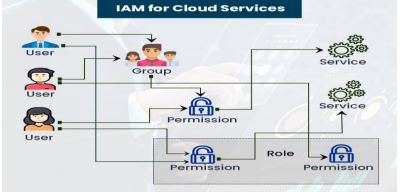
\includegraphics[width=1\textwidth]{gfx/Picture/IAMISH.PNG}
 \caption{IAM für Cloud Dienste \cite{Moha19, S.3}}
 \label{fig:IMAISH}
\end{figure}
Dies ist ein Beispiel, wie die oben genannten Punkte umgesetzt werden können.
Dabei haben die Accounts der Personen entweder direkte Berechtigung oder diese werden mittels Gruppen verteilt.
Sobald der Account die Berechtigung hat, kann dieser auf die dahinter steckende Ressource zugreifen.
Die Berechtigungen können dabei auch mittels Profile zusammengefasst werden.
Die Grafik (\ref{fig:IMAISH}) stellt dies dar.
\newline
Dabei kann dies auf verschiedenen Wegen umgesetzt werden, da dieselbe Lösung für gewisse Fälle nicht funktioniert.
Zum Beispiel beschreibt \cite{Cal17, S.208} das Problem, wie die United States of America am besten mit ihren Verbündeten kooperieren sollten.
Da es sich dabei um sensitive Informationen handelt, welche an verschiedene Partner vermittelt werden, muss der Zugriff reguliert werden.
Auch haben die verschiedenen Länder unterschiedliche Gesetze, worauf geachtet werden muss. 
Deswegen gibt es keine universelle Methode, um eine solche Herausforderung zu lösen. \cite{Cal17, S.208}


\subsection{Vergleich mit Datenbanken}
\label{sec:chapter04:DB}
Die Helvetia verwendet zum Speichern der Informationen für die Berechtigungsstruktur sogenannte HV-Tabellen.
Bei diesen HV-Tabellen handelt es sich, um DB2-Tabellen.
Zudem besteht eine Ähnlichkeit zwischen dem Nutzer und dem Profil in der Berechtigungsstruktur im Vergleich zum Account und der Gruppe in Datenbanken.
Deswegen wird betrachtet, wie der Standard von Accounts und Gruppen innerhalb von Datenbanken ist.
\newline
Berechtigungen für Rollen werden mittels folgenden Kommand vergeben: 
\newline
\newline
GRANT...ON...TO...[GRANT OPTION]
\newline
\newline
Dabei wird für die spezifische Berechtigung, zum Beispiel eine View und einen Account oder eine Gruppen angegeben.
Zudem kann auch hinzugefügt werden, ob die Rolle die Berechtigung hat, anderen Accounts die Berechtigungen zu geben.\cite{Ram09, S.474-475}
\newline
Wenn man sich zum Beispiel das Bild (\ref{fig:Berch}) ansieht, könnte der Befehl wie folgt aussehen:
\newline
\newline
GRANT UPDATE ON PKU$00$ TO USER$895$.
\newline
\newline
Das würde in diesem Beispiel bedeuten, dass der Nutzer USER$895$ die Bearbeitungsberechtigung für die Ressource PKU00 erhalten hat.
Dabei ergibt sich die Frage auf, was bevorugt verwendt werden sollte:
\newline
Eine individuelle Berechtigungsvergabe oder Gruppenvergabe für die Accounts.
Microsoft hat folgendes als Best Practice definiert:
\newline
\newline
\textit{"`To simplify administration, create groups and assign each group permission to functional areas and model objects.
You can then add and remove users from the groups without accessing the Master Data Manager UI.
\newline
\newline
Do not assign additional permissions to an individual user, and do not include a user in multiple groups that have access to Master Data Manager. In addition, do not use hierarchy member permissions unless you want a group to have limited access to specific members."'} \cite{Micro}
\newline
\newline
Microsoft gibt an, dass man Gruppen erstellen soll.
Die individuellen Nutzer sollen dabei keine zusätzlichen Berechtigungen bekommen.
Ebenso ist es wichtig, dass diese nicht in mehreren Gruppen sind, welche Zugriff auf den Master Data Manager haben.
Und auch IBM gibt in seiner Best Practice an, dass Angestellte in einem Unternehmen mittels Gruppen organisiert werden sollten. \cite{IBMGroup}
\newline
Dies ist jedoch in der Praxis schwierig umzusetzen.
Im Idealfall benötigt jeder Mitarbeiter ein oder zwei Standardprofile, welche dem Nutzer alle Berechtigungen geben.
Dies ist aber selten der Fall, da die Nutzer nach beispielsweise einem halben Jahr an einem anderen Projekt arbeiten und daher andere Berechtigungen benötigen.
Wenn man für jeden solchen Fall ein neues Standardprofil erstellt, werden diese unübersichtlich.
Ebenso würde das Konzept der Standardprofile in Frage gestellt werden, wenn die Anzahl dieser Standardprofile der Anzahl der Berechtigungen gleicht.
Dennoch sollte es versucht werden, dass Nutzer so wenig zusätzliche Berechtigungen wie möglich bekommen, um Best Practice Standards einzuhalten. 

\section{DSGVO}
\label{sec:chapter04:DSGVO}
Neben den technischen Herausforderungen und Anforderungen muss die Struktur neben dem \ac{VAIT} auch den Standards der \ac{DSGVO} erfüllen.
Bei Verstoß gegen diese kann es zur Verwarnung bis zum endgültigen Verbot der Datenverarbeitung kommen. \cite{EuroK}
Dies würde die Helvetia sehr viel Geld kosten, da diese nicht mehr operieren könnte.
\newline
Eine sichere Berechtigungsstruktur ist daher nötig, um diese Anforderung der \ac{DSGVO} zu befriedigen.
Diese ist nämlich verletzt, wenn Daten, für die das Unternehmen verantwortlich ist, in ihrer Vertraulichkeit, Verfügbarkeit oder Integrität verletzt werden.
Deswegen sind Mitarbeiter, die mehr Berechtigungen haben als jene, die sie wirklich benötigen, eine Risikostelle. \cite{EuroW}
\newline
Daher sollte die neue Berechtigungsstruktur so gestaltet werden, dass die Verständlichkeit, Verfügbarkeit und INtegrität der Daten nicht verletzt werden können.

\section{Herausforderung und Anforderungen}
\label{sec:chapter04:Herausforderung}
Bei der Recherche (\ref{ch:Recherche}) sind verschiedene Herausforderungen und Anforderungen aufgetreten.
Um qualitativ ein Konzept entwickeln zu können, müssen diese Herausforderungen und Anforderungen aufgelistet und analysiert werden.
Neben den genannten Punkten wurde der Punkt Implementierung hinzugefügt, da diese bei der Entscheidung der Konzepte elementar ist.
Das Unternehmen muss dabei über die Kosten des neuen Konzepts und dessen Performance bewusst sein.
\begin{itemize}
	\item Performance der Tabellen erhöhen 
	\item Übersichtlichkeit erhöhren (effizientere Verifizierung der Mitarbeiter)
	\item Rekursive Beziehungen verhindern
	\item Hierarchien verringern
	\item \ac{K/W}
	\item Implementierung
\end{itemize}
Eine Quantifizierung findet mittels Prioritätsanalyse (\ref{fig:Prio}) statt, um festzustellen wie die Prioritäten der Konzepte zu bewerten sind. \cite{BdIufH}
Bei der Prioritätsanalyse wurde sich für ein vier Punktesystem entschieden.
\newline
Im Vergleich zwischen der Performance und der Übersichtlichkeit, wurden der Performance drei Punkte gegeben und die Übersichtlichkeit hat nur einen Punkt erhalten, da die Performance eine der Grundanforderungen ist, weswegen die Berechtigungsstruktur geändert werden soll.
Die Übersichtlichkeit dazu ist weniger wichtig.
Die Performance und die Rekursion haben jeweils zwei Punkte bekommen, da eine performante Struktur keine rekursiven Beziehungen enthält.
\ac{K/W} sowie Performance haben jeweils zwei Punkte bekommen.
Dies liegt daran, dass neben der Performance die \ac{K/W} elementar sind, da eine Struktur, die sich kaum warten lässt, mehr Ressourcen in der Zukunft kosten wird.
Zwischen der Übersichtlichkeit und der Rekursion wurden der Rekursion drei Punkte gegeben und der Übersichtlichkeit nur einen, weil rekursive Strukturen unübersichtlicher sind und es daher wichtiger ist, dass es keine gibt.
Übersichtlichkeit und Hierarchie haben beide zwei Punkte erhalten, da beide eine gleiche Rolle bei der Lesbarkeit der Struktur spielen.
Übersichtlichkeit sowie Rekursion und Hierarchie bekommen einen Punkt im Vergleich zu \ac{K/W}, weil dieser Punkt langfristig eine wichtige Rolle spielt, und die anderen drei Punkte sollten keine Probleme sein, sofern sich an die Konventionen gehalten wird, damit die Struktur wartbar bleibt.
Die Rekursion bekommt zur Hierarchie vier Punkte und die Hierarchie zur Rekursion null Punkte, da eine rekursive Beziehung die Hierarchie automatisch unendlich macht.
\newline
\newline
Wenn man dies auswertet, bekommt die Performance einen Gewichtsfaktor von 16,67\%, die Übersichtlichkeit 20,00\%, die Rekursion 18,33\%, die Hierarchie 6,67\%, die \ac{K/W} 18,33\% und Implementierung 20,00\%.
Dadurch sieht die Rangfolge wie folgt aus:
\begin{enumerate}
	\item Implementierung | Übersichtlichkeit
	\item Rekursion | \ac{K/W}
	\item Performance
	\item Hierarchie
\end{enumerate}
Anhand dieser Reihenfolge werden die folgenden Konzepte entwickelt.
\newpage
\begin{figure}[h!]
\hspace*{-2cm}
 \centering
 \includegraphics[width=1.25\textwidth]{gfx/Picture/Prioritatätsanalyse.PNG}
 \caption{Prioritätsanalyse der Kriterien}
 \label{fig:Prio}
\end{figure}

\section{Konzept hierarchische Struktur}
\label{sec:chapter04:Struktur}
\begin{figure}[h!]
 \centering
 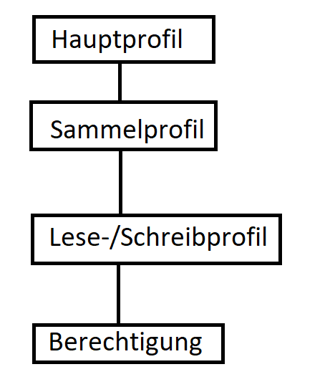
\includegraphics[width=0.75\textwidth]{gfx/Picture/Hierarchie.PNG}
 \caption{Hierarchieaufbau für das Konzept hierarchische Struktur}
 \label{fig:Struktur}
\end{figure}
Das erste Konzept für die Struktur ist wie folgt aufgebaut.
Wie man in der Grafik (\ref{fig:Teil}) aus dem zweiten Kapitel erkennen kann, gibt es bei der aktuellen Berechtigungsstruktur keine Struktur.
Um dementsprechend die genannten Problem zu beheben, wurde die neue Struktur (\ref{fig:Struktur}) entwickelt.
Um die \ac{K/W} zu verbessern, wurden die folgenden Konventionen für dieses Konzept entwickelt.
Es it dabei anzumerken dabei ist, dass die Durchsetzung und Implementierung dieser Konventionen trotzdem keinen unerheblichen Aufwand darstellt.
\begin{itemize}
	\item Profile enthalten nur noch Profile oder Berechtigungen.
	\item Die Berechtigungsstruktur soll nur noch eine Hierarchietiefe von maximal vier haben.
	\item Die erste Hierarchiestufe enthält das Standardprofil, welches dem Nutzer gegeben wird.
	\item Die zweite Hierarchiestufe enthält die jeweiligen Sammellese- und -schreibprofile, die jeweils in die Fachbereiche getrennt sind.
	\item Die dritte Hierarchiestufe enthält die individuellen Lese- und Schreibprofile.
	\item Die vierte Stufe enthält die Berechtigungen.
	\item Manche der bestehenden Profile beinhalten aktuell, was zukünftig Hauptprofile wären.
In solchen Fällen würden diese Profile zu Hauptprofilen werden und vom vorherigen Hauptprofil separiert werden.
	\item Manche Fachbereiche haben aufzählende Profile (\ref{fig:Profile}).
Diese Profile sollen nur noch die Berechtigungen für den eigenen Vorgang enthalten, sodass ein Privas Profil nur Privas Berechtigungen enthält.
Die Berechtigungen, die verloren gehen, würden eigene Profile bekommen und so über ein anderes Sammelprofil dem Hauptprofil hinzugefügt werden.
	\item Sollte ein Nutzer weitere Berechtigungen benötigen, würden ihm diese direkt zugewiesen werden.
	\item Wenn ein Account reaktiviert wird, muss dieser rezertifiziert werden.
\end{itemize}
Diese Konventionen sollen verhindern, dass die Struktur weiter wächst und dass man ohne Probleme feststellen kann, was für Berechtigungen ein Profil hat.
Zudem hat es den Vorteil, dass rekursive Beziehungen, sowie redundante Berechtigungsvergabe nicht möglich sind, da die Profile nur noch Profile oder Berechtigungen enthalten, die nicht mehr auf sich gegenseitig zeigen.
Dadurch soll auch die Übersichtlichkeit verbessert und das Hierarchieproblem auf ein Minimum gebracht werden.
Außerdem sollte die Performance verbessert werden.
Dabei helfen verschiedene Faktoren, um diese zu verbessern.
Die reduzierte der rekursiven Beziehungen, sowie die Vereinfachung der Struktur, mit der Reduktion der Berechtigungen, machen die Berechtigungsstruktur performanter.
\begin{figure}[h!]
\hspace*{-2cm}
 \centering
 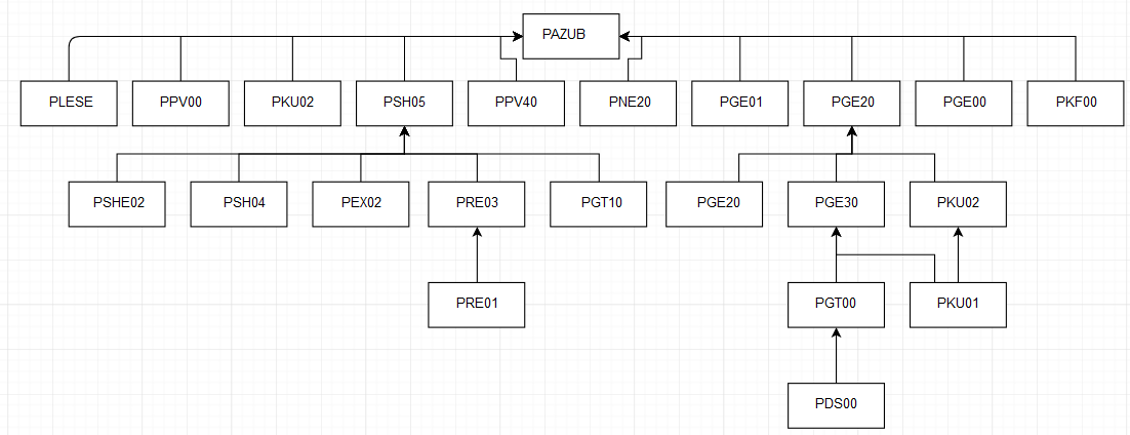
\includegraphics[width=1.25\textwidth]{gfx/Picture/Vorher.PNG}
 \caption{Beispiel der bestehenden Berechtigungsstruktur}
 \label{fig:AltBer}
\hspace*{-2cm}
 \centering
 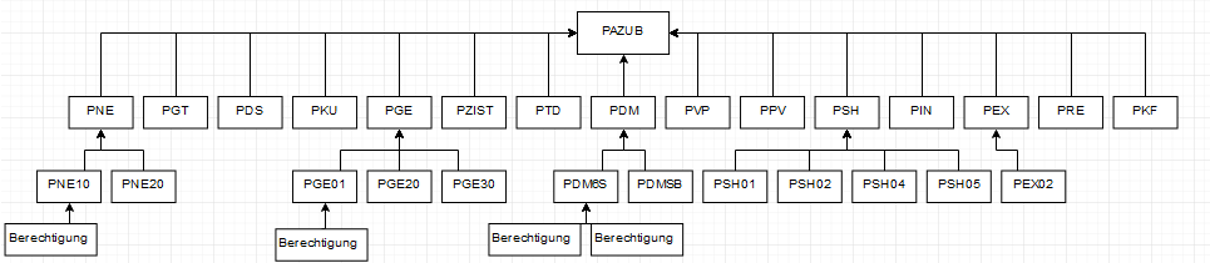
\includegraphics[width=1.25\textwidth]{gfx/Picture/Nachher.PNG}
 \caption{Beispiel der neuen Berechtigungsstruktur}
 \label{fig:NeuBer}
\end{figure}
Das Bild (\ref{fig:AltBer}) zeigt eine bestehende Berechtigungsstruktur.
(\ref{fig:NeuBer}) hingegen bildet die Struktur nach den neuen Konventionen dar.
Diese beide Bilder wurden den IT-Spezialisten gezeigt, die befragt wurden.
Einheitlich haben alle befragten IT-Spezialisten angegeben, dass Sie die neue Struktur übersichtlicher finden und diese einfacher zu verstehen ist.
Zudem wurde kann auch erkannt werden, dass die Hierarchie verringert wurde.
\newline
Das aktuelle Verfahren, das verwendet wird, um die Berechtigung zu überprüfen, gleicht einem Insertion-Sort.
Dabei wird jedes einzelne Profil durchgegangen, bis die gewünschte Berechtigung gefunden wurde.
Dies weißt eine Komplexität von n im Optimalfall und $n^2$ im schlimmsten Falle auf.
n beschreibt dabei die Anzahl von Profilen/Berechtigungen, die der Algorithmus durchlaufen muss. \cite{log, S.12, weblogMer}
\newline
Bei der neuen Struktur kann ein Merge-Sort genutzt werden.
Dabei achtet der Algorithmus auf bestimmte Eigenschaften der Profile.
Würde zum Beispiel verlangt werden, dass der Nutzer eine Berechtigung für PNE10 hat, würde nur der Baum von PNE durchsucht werden und in diesem Falle direkt PNE10 ausgewählt werden.
Dieser Suchalgorithmus ist komplexer als der Insertion-Sort. Er ist jedoch deutlich effizienter bei einer größeren Menge von Profilen und Berechtigungen.
Die Komplexität beläuft sich bei ihm auf n*log(n) im besten, wie auch im schlechtesten Fall. \cite{log, S.12, weblogMer} 
\newline
Wenn beispielsweise n = $100$ wäre, würden die Ergebnisse wie folgt aussehen:
\newline
\newline
Best-Case(Insert) = $100$
\newline
Worst-Case(Insert) = $100^2 = 10.000$
\newline
\newline
Best-Case(Merge) = $100*log(100) = 200$
\newline
Worst-Case(Merge) = $100*log(100) = 200$
\newline
\newline
Wie man erkennen kann, ist der neue Algorithmus im Best-Case langsamer, aber im Worst-Case deutlich schneller und bietet allgemein eine konsistente Zeit, welche für eine Versicherung wichtig ist.
Der Insertion-Sort sowie der Merge-Sort haben auch eine average Formel: \cite{weblogMer,weblogIn}
\newline
\newline
Average(Insert) = $100^2 = 10.000$
\newline
\newline
Average(Merge) = $100*log(100) = 200$
\newline
\newline
Man kann erkennen, dass im normalen Fall die neue Struktur mit dem Merge-Sort deutlich effektiver ist als die bestehende Struktur.
Diese würde durchschnittlich $50$ mal effektiver sein.
\newline
\newline
Die Entwicklung dieses Konzeptes ist aufwendig und komplex.
Es gibt dabei zwei Möglichkeiten, wie dieses umgesetzt werden kann.
Die erste Möglichkeit besteht darin, dass sich eine Gruppe von Entwicklern an die bestehende Struktur setzen, eine Kopie davon erstellen und anhand der Kopie die neue Struktur erstellen.
Dies ist jedoch zeitaufwändig und es besteht ein hohes Potenzial, dass Fehler durch nachlässiges Arbeiten geschehen.
\newline
Die zweite Möglichkeit wäre ein Algorithmus zu schreiben, welcher dies automatisiert.
Da weder die Zeit besteht noch die entsprechende Umgebung zum Testen eines Prototypen, kann die Entwicklung des Algorithmus innerhalb dieser Arbeit nur mithilfe Pseudocode stattfinden.
Dabei würde die Automatisierung wie folgt aussehen.
\newline
\newline
\textbf{Algorithmus} conversionToNewStructure(DB$2$ T)
\newline
\newline
\textbf{Input} Eine DB2 Tabelle T, welche die Struktur enthält
\newline
\newline
\textbf{Output} Neue DB2 Tabelle NT, welche die neue Struktur von Profilen enthält.
\newline
\newline
Der Algorithmus muss dabei die Profile in zwei Kategorien aufteilen:
\begin{itemize}
	\item Standardprofil
	\item Lese-/Schreibprofil
\end{itemize}
Für die Standardprofile werden die Profile überprüft, die viele Unterprofile haben.
Wenn ein Profil XY viele Unterprofile hat, wird dieses zu einem Standardprofil.
Die restlichen Profile werden zu Lese-/Schreibprofile.
Die individuellen Sammelprofile werden basierend auf den Lese-/Schreibprofilen generiert.
Die Verbindungen zwischen den bisherigen Profilen werden aufgebrochen und zu den neuen Sammelprofilen zugewiesen, welche mit dem Standardprofil verbunden sind.
Anschließend werden auf redundante Profile und Berechtigungen überprüft, welche dann entfernt wird.
Dabei muss man aber zum Schluss begutachten, ob alle generierten Standardprofile wirklich Standardprofile sein sollten sowie ob die bestehende Anzahl ausreichend ist.
Die Grafik (\ref{fig:Hier}) stellt dies als Ablaufdiagram dar.
\begin{figure}[h!]
 \centering
 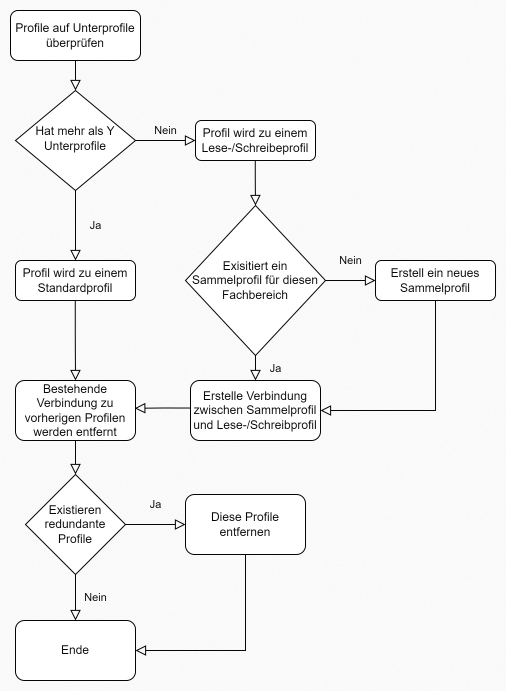
\includegraphics[width=0.77\textwidth]{gfx/Picture/Hier.PNG}
 \caption{Ablaufdiagram für das hierarchische Struktur Konzept}
 \label{fig:Hier}
\end{figure}
\newpage
\section{Konzept minimalistische Struktur}
\label{sec:chapter04:minimal}
Im Gespräch der IT-Spezialisten kam der Vorschlag auf, dass man einen minimalistischen Ansatz nutzen könnte.
Dabei haben die IT-Spezialisten folgende Vorschläge für die Konventionen gemacht:
\newline
\begin{itemize}
	\item Profile enthalten nur noch Profile oder Berechtigungen.
	\item Es werden Standardprofile für die jeweiligen Abteilungen entwickelt.
	\item Nutzer, die in verschiedenen Abteilungen operieren, erhalten die jeweiligen Standardprofile.
	\item Zusätzliche Berechtigungen werden dem Nutzer direkt zugeordnet.
	\item Wenn ein Account reaktiviert wird, muss dieser rezertifiziert werden.
\end{itemize}
\begin{figure}[h!]
 \centering
 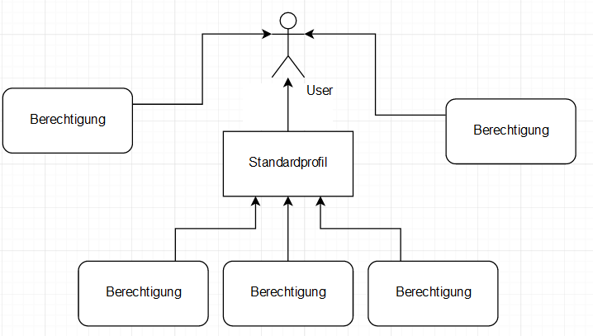
\includegraphics[width=1\textwidth]{gfx/Picture/Minimal.PNG}
 \caption{Darstellung für das Konzept minimalistische Struktur}
 \label{fig:Min}
\end{figure}
Die IT-Spezialisten fanden auch, dass dies übersichtlicher als die bestehende Struktur ist.
Dieses Konzept hat den Vorteil, dass es kaum noch eine Hierarchie gibt.
Dadurch entfällt das Problem der Rekursion sowie redundanter Berechtigungsvergabe.
Die \ac{K/W} ist einfacher in diesem Sinne, da nur überprüft werden muss, ob die Standardprofile über die notwendigen Berechtigungen verfügen.
Auf der anderen Seite ist die Entwicklung aufwendig, da erst einmal bestimmt werden muss, welche Berechtigungen für einen Fachbereich notwendig sind. Ebenso muss sichergestellt werden, dass alle Nutzer ihre Berechtigungen beibehalten.
Es besteht nämlich die Gefahr, dass bei dem Wechsel Berechtigungen verloren gehen.
\newline
\newline
Wenn man (\ref{fig:Min}) betrachtet, kann für diese Struktur nur ein Insertion-Sort verwendet werden.
Dies liegt daran, dass der Sort die individuellen Einträge durchlesen muss, da es keine Information gibt, wo welche Berechtigung ist.
Die aktuelle Struktur verwendet auch einen Insertion-Sort, aufgrund des gleichen Problems.
Jedoch ist zu bemerken, dass die Anzahl der \textit{n} bei diesem Konzept geringer ist, da es nicht die verschiedenen Profile mit Redundanzen gibt.
\newline
\newline
Ein Hauptprofil hatte zum Beispiel $110$ Profile mit enthalten Berechtigungen.
Von diesen $110$ waren $78$ redundante Profile.
Da Profile eine Ansammlung von Berechtigungen sind, ist die Anzahl von redundanten Berechtigungen deutlich höher.
Wenn man nur zwischen der bestehenden Struktur mit der minimalistischen Struktur unterscheidet, erhält man folgenden Vergleich:
\newline
\newline
Best-Case(Alte Struktur) = $110$
\newline
Worst-Case(Insert) = $110^2 = 12.100$
\newline
Average(Insert) = $110^2 = 12.100$
\newline
\newline
Best-Case(Neue Struktur) = $32$
\newline
Worst-Case(Neue Struktur) = $32^2 = 1.024$
\newline
Average(Neue Struktur) = $32^2 = 1.024$
\newline
\newline
Man kann feststellen, dass obwohl die neue Struktur nicht über einen effizienteren Algorithmus verfügt, dieser trotzdem eine bessere Performance hat.
Die neue Struktur wäre in diesem Beispiel ca. $12$ mal performanter als die bestehende Struktur.
\newline
\newline
Ebenso kann für dieses Konzept eine manuelle Lösung sowie auch eine automatische verwendet werden.
Wie im vorherigen Fall kann eine Kopie vom vorherigen Konzept erstellt werden, welches dann in das neue Konzept modeliert wird.
Jedoch wird der Prozess der individuellen Berechtigungsvergabe zu den einzelnen Nutzern zeitaufwendig sein.
Dabei können auch Berechtigungen verloren gehen, was dringend zu vermeiden ist.
\newline
Als Alternative kann ein Algorithmus verwendet werden.
Dieser ist dem vorherigen in der Grundstruktur gleich:
\newline
\newline
\textbf{Algorithmus} conversionToNewStructure(DB$2$ T)
\newline
\newline
\textbf{Input} Eine DB2 Tabelle T, welche die Struktur enthält
\newline
\newline
\textbf{Output} Neue DB2 Tabelle NT, welche die neue Struktur von Profilen enthält.
\newline
\newline
Der Algorithmus würde die komplette bisherige Struktur auseinanderbrechen.
Anschließend werden die Standardprofile anhand der Fachbereiche neu geformt und den Nutzern der jeweiligen Bereiche zugewiesen.
Die bisherigen Berechtigungen werden anschließend den Nutzern direkt angehängt.
Redundate Berechtigungen werden entfernt.
Die Grafik (\ref{fig:Mini}) stellt dies als Ablaufdiagram dar.
\begin{figure}[h!]
 \centering
 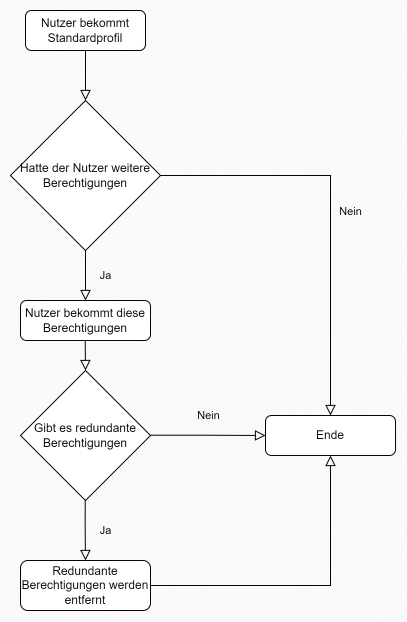
\includegraphics[width=1\textwidth]{gfx/Picture/Mini.PNG}
 \caption{Ablaufdiagram für das Minimalistisch Konzept}
 \label{fig:Mini}
\end{figure}